%!TEX root = ../masters.tex

\chapter{Metodologia}
\label{cha:methodology}

Este trabalho tem como metodologia uma pesquisa de caráter não-experimental e quantitativa, por se tratar de extração automática de metadados por ferramentas previamente selecionadas, tendo os resultados comparados com a extração manual do mesmo conjunto de artigos científicos.

% Explicar o passo a passo que será utilizado

Primeiramente, são filtradas as ferramentas encontradas a fim de analisar realmente as que possuem viabilidade técnica de testes dentro do objetivo da pesquisa. Desta forma, diversos elementos serão utilizados a fim de obter os resultados desejados.

% Explicar de modo geral como será o processo

De modo geral o procedimento de testes deste trabalho será realizado através da instalação e execução de cada ferramenta selecionada, permitindo que cada uma tenha seu conjunto necessário de tecnologias para seu correto funcionamento. Assim, os artigos selecionados para testes serão utilizados em cada uma destas ferramentas e seus resultados analisados, centralizados e consolidados a fim de se obter uma conclusão para cada análise encontrada. O fluxo de passos necessários para a realização destes testes pode ser melhor visualizado na \autoref{fig:metodology}.

\begin{figure}
    \centering
    \caption{Processo de Metodologia utilizado}
    \label{fig:metodology}
    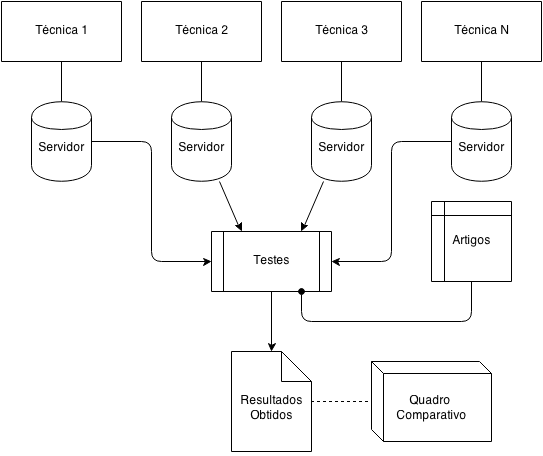
\includegraphics[width=0.8\linewidth]{./assets/images/metodology}
    \center\footnotesize{Fonte: O próprio autor}
\end{figure}


\section{Escolha do Corpus}
\label{sec:corpus}

% Falar da seleção de artigos de várias áreas

Visando provar a eficiência das ferramentas - juntamente com a implementação das técnicas por elas utilizadas -, desejamos ter resultados exatos da extração de metadados, de maneira que possam ser comparados e verificados com os metadados manualmente extraídos. Deste modo, foi selecionada uma série de artigos científicos das mais diversas áreas de pesquisa, com padrões visuais distintos.

% Porque selecionar artigos de diferentes áreas

Em virtude da necessidade de realizar testes com as ferramentas selecionadas em um ambiente real e representativo, foi realizada uma pesquisa no site do CNPq \url{http://www.cnpq.br/} a fim de obter a relação das áreas e subáreas do conhecimento reconhecidas oficialmente. Deste modo foi constatada a existência de 9 (nove) áreas do conhecimento, totalizando 1.288 (mil duzentas e oitenta e oito) subáreas, conforme pode ser verificado na \autoref{tab:areas-cnpq}.

\begin{table}
    \caption{Áreas do Conhecimento (CNPq)}
    \begin{center}
        \begin{tabular}{|l|c|}
            \hline 
            \textbf{Áreas do Conhecimento} & \textbf{Subáreas} \\ 
            \hline 
            Ciências Agrárias & 157 \\
            Ciências Biológicas & 104 \\
            Ciências da Saúde & 76 \\
            Ciências Exatas e da Terra & 243 \\
            Ciências Humanas & 163 \\
            Ciências Sociais Aplicadas & 185 \\
            Engenharias & 305 \\
            Lingüística, Letras e Artes & 53 \\
            Outros & 4 \\
            \hline
            \textbf{Total} & \textbf{1288} \\
            \hline
        \end{tabular}
    \end{center}
    \center\footnotesize{Fonte: \url{http://www.memoria.cnpq.br/areasconhecimento/index.htm}}
    \label{tab:areas-cnpq}
\end{table}

Com base no grande número de subdivisões de cada área do conhecimento (vide \autoref{tab:areas-cnpq}), a seleção das subáreas será limitada a 2 (duas), sendo a escolha feita com base na existência de curso de graduação e/ou departamento na Universidade Federal de Minas Gerais (UFMG), o que facilitaria o contato com professores e coordenadores dos respectivos cursos. Desta forma, excluindo-se a área ``Outros'', seriam analisadas 16 (dezesseis) subáreas, sendo 2 (duas) para cada uma das 8 (oito) áreas do conhecimento.

Com as subáreas selecionadas, foi realizada uma entrevista com professores e/ou coordenadores de cada curso ou departamento correspondente na UFMG, obtendo então as bases de dados e/ou revistas mais utilizadas e relevantes para cada subárea do conhecimento, construindo um \emph{corpus} realmente significativo. A relação dos professores entrevistados e as subáreas do conhecimento selecionadas pode ser vista na \autoref{tab:subareas-professores}.

\begin{table}
    \caption{Professores entrevistados para cada subárea do conhecimento.}
    \begin{center}
        \begin{tabular}{|p{6cm}|p{8cm}|}
            \hline 
            \textbf{Subárea do Conhecimento} & \textbf{Professor(a)}\\ 
            \hline 
            Arquitetura e Urbanismo & Eleonora Sad de Assis \\
            \hline
            Ciência da Computação & Adriano Alonso Veloso \par 
                                    Alberto Henrique Frade Laender \par 
                                    Arnaldo de Albuquerque Araújo \\
            \hline
            Ciência da Informação & Beatriz Valadares Cendón \\
            \hline
            Ciências Biológicas (Genética) & Mônica Bucciarelli Rodriguez \\
            \hline
            Ciências Biológicas (Zoologia) & Alfredo Hannemann Wieloch \\
            \hline
            Enfermagem & Eline Lima Borges \par
                         Tania Couto Machado Chianca \par
                         Daclé Vilma Carvalho \\
            \hline
            Engenharia Civil & Antônio Neves de Carvalho Júnior \\
            \hline
            Engenharia Mecânica & Antônio Eustáquio de Melo Pertence \par
                                  Alexandre Mendes Abrao \\
            \hline
            Fonoaudiologia & Sirley Alves da Silva Carvalho \\
            \hline
            Geologia & Adolf Heinrich Horn \\
            \hline
            História & Adriana Romeiro \\
            \hline
            Letras & Adriana Silvina Pagano \\
            \hline
            Medicina Veterinária & João Paulo Amaral Haddad \par
                                   Jenner Karlisson Pimenta dos Reis \\
            \hline
            Música & João Pedro Paiva de Oliveira \\
            \hline
            Psicologia & Carmen Elvira Flores-Mendoza Prado \par
                         Livia de Oliveira Borges \\
            \hline
            Zootecnia & Ângela Maria Quintão Lana \\
            \hline
        \end{tabular}
    \end{center}
    \label{tab:subareas-professores}
\end{table}

Para cada uma das subáreas do conhecimento selecionadas foram coletados 7 (sete) artigos científicos. Em virtude da diversidade de quantidade de bases de dados informadas pelos professores de cada subárea do conhecimento (\autoref{tab:databases}), a pesquisa foi limitada a 2 (duas) bases, na ordem apresentada pelos próprios pesquisadores, contemplando 4 (quatro) artigos para a primeira base e 3 (três) para a segunda. Para a subárea ``Ciências Biológicas (Genética)'' somente uma base de dados será utilizada, portanto dela serão retirados os 7 artigos necessários. No total foram selecionados 112 (cento e doze) artigos, contemplando 16 subáreas do conhecimento e 32 bases de dados, formando então o \emph{corpus} utilizado como base desta pesquisa.

\begin{table}
    \caption{Bases de Dados informadas pelos professores entrevistados, por subárea do conhecimento.}
    \begin{center}
        \begin{tabular}{|p{6cm}|p{8cm}|}
            \hline 
            \textbf{Subárea do Conhecimento} & \textbf{Bases de Dados} \\ 
            \hline 
            Arquitetura e Urbanismo & Scielo, Web of Science, Scopus \\
            \hline
            Ciência da Computação & DBLP, ACM Digital Library, IEEE Xplore \\
            \hline
            Ciência da Informação & LISA, ISTA, LISTA \\
            \hline
            Ciências Biológicas (Genética) & PubMed \\
            \hline
            Ciências Biológicas (Zoologia) & Zoological Records, Biological Abstracts \\
            \hline
            Enfermagem & MedLine, Lilacs, CINAHL, EBSCO, IBECS, BDENF \\
            \hline
            Engenharia Civil & Construction and Building Materials (ELSEVIER), Cement and Concrete Composites (ELSEVIER), Composites Science and Technology (ScienceDirect), Cement and Concrete Research (ELSEVIER), Materials Research (Scielo) \\
            \hline
            Engenharia Mecânica & Scopus, ScienceDirect, Web of Science, SpringerLink, Elsevier, Research Gate \\
            \hline
            Fonoaudiologia & Pubmed, Bireme \\
            \hline
            Geologia & Springer, Scielo, Portal CAPES \\
            \hline
            História & Scielo, Jstor, Redalyc \\
            \hline
            Letras & Delta (Scielo), Periódicos Letras UFMG, Periódicos UFSC \\
            \hline
            Medicina Veterinária & PubMed, Scielo \\
            \hline
            Música & RISM, RILM, JSTOR, Grove Dictionary of Music \\
            \hline
            Psicologia & Scopus, PsycInfo, Scopus, Psicodoc \\
            \hline
            Zootecnia & Dairy Science, Animal, Poutry Science \\
            \hline
        \end{tabular}
    \end{center}
    \label{tab:databases}
\end{table}

A seleção dos artigos em cada base de dados foi feita de maneira arbitrária, levando em consideração diferenças de leiautes e posicionamento dos elementos, permitindo que uma maior variedade de documentos seja analisada.

% Artigos em Inglês, somente

Todos os artigos selecionados foram escritos na língua inglesa. Esta decisão foi tomada em virtude de, além de ser a língua inglesa a universal para disseminação de conhecimento, ela é a mais utilizada no meio acadêmico, possuindo um universo muito maior e mais rico de artigos escritos no idioma. Além disso, algumas das ferramentas e respectivas técnicas utilizadas nos testes utilizam de ``processamento de linguagem natural'' para extração dos metadados, tendo por padrão a utilização do inglês na análise dos textos dos documentos.

Em virtude destas colocações a abrangência de outros idiomas entraria em um aspecto que não é objetivo deste trabalho abordar, visto a diversificação de culturas e símbolos, fazendo com que línguas orientais, como o mandarim ou japonês por exemplo, tenham análises diferenciadas em função de suas diferenças nas formas de representação e leitura, necessitando de outras técnicas e/ou ferramentas mais direcionadas a fim de obter os resultados esperados.

No que tange a escolha das ferramentas para testes foi utilizado apenas um ponto na seleção: a sua utilização por linha de comando (\emph{command line}). Embora algumas ferramentas possuem código aberto a extração de metadados faz parte de um contexto específico da aplicação, dificultando a utilização de apenas este recurso. Assim, foram selecionadas para testes apenas as ferramentas que permitem o uso de sua funcionalidade de extração de metadados de maneira individual, independente da linguagem de programação ou tecnologia apresentada. 

Deste modo, dentre as ferramentas apresentadas neste trabalho, presentes na \autoref{tab:tools-consolidated}, as ferramentas selecionadas para teste foram: Cermine, CiteSeer, CrossRef e ParsCit.
    

\section{Desenho do Experimento}
\label{sec:experiment-design}

Tendo selecionadas as ferramentas e os artigos que serão utilizados para os testes, parte-se para a instalação adequada de cada ferramenta, juntamente com as tecnologias necessárias e as linguagens de programação utilizadas pelos seus desenvolvedores. 

Cada ferramenta será testada em separado, observando suas características particulares. Assim, cada artigo selecionado será testado para aquela ferramenta, anotando os resultados obtidos na extração. Estes resultados serão separados por metadados, o que permitirá calcular qual a porcentagem de acerto que cada ferramenta teve na extração de cada metadado analisado.

Assim, o processo será repetido para cada ferramenta e o resultado registrado, permitindo calcular sua porcentagem total de acertos de maneira simplificada. Para isso será criado um ``Quadro Comparativo'', no qual serão inseridos os resultados dos testes de cada ferramenta. 

\subsection{Metadados, Pesos e Resultados}
\label{ssec:metadata-results}

% Importância de se ter pesos em função dos metadados

Em se tratando de pesquisa por artigos científicos, pequenos detalhes podem fazer a diferença. Desta forma, uma extração de metadados não muito eficaz pode prejudicar direta ou indiretamente os resultados apresentados por esta busca. Por outro lado, alguns metadados tendem a ser mais utilizados na pesquisa que outros, o que implica em uma responsabilidade maior na eficiência de sua extração. 

% Quais metadados são mais importantes para uma pesquisa de artigos

Geralmente quando vamos buscar artigos, procuramos primeiro pelo título (quando procuramos por um documento específico) ou então pelo nome do autor (quanto procuramos por artigos de um determinado pesquisador). Deste modo serão atribuídos pesos para cada um dos metadados, de maneira a valorizar a extração destas informações que podem influenciar diretamente os resultados de busca.

Deste modo apresentamos a \autoref{tab:metadata-weight}, que demonstra como cada metadado deve ser interpretado e qual o peso que lhe será atribuído, sendo utilizado o inteiro 1 (um) para o peso mais baixo e o 5 (cinco) para o peso mais alto, sendo consequentemente o(s) metadado(s) mais importante(s). Os pesos utilizados, assim como a ordem de importância escolhida foram fundamentados de maneira arbitrária, baseados na experiência do autor.

% Tabela de metadados e pesos

\begin{table}
    \caption{Os metadados e seus pesos atribuídos}
    \begin{center}
        \begin{tabular}{|p{3cm}|p{8cm}|C{1cm}|}
            \hline \textbf{Metadado} & \textbf{Relevância} & \textbf{Peso} \\ 
            \hline Título & Um dos termos mais buscados quando se pesquisa um artigo & 5 \\
            \hline Autor(es) & Outro termo muito utilizado na busca por artigos & 4 \\
            \hline E-mail(s) & Pouco relevante no quesito pesquisa de artigos & 1 \\
            \hline Resumo & Importante por conter palavras chaves e o resumo propriamente dito & 3 \\
            \hline Referências & Muito importante e necessário, pois será utilizada na referência inversa de autores & 4 \\
            \hline 
        \end{tabular} 
    \end{center}
    \label{tab:metadata-weight}
\end{table}

Como a extração de um metadado nem sempre ocorre de maneira 100\% eficaz, visando uma avaliação mais detalhada de cada ferramenta, será calculada a precisão do resultado da extração de cada metadado, feita com base na porcentagem de sucesso obtida para aquele conjunto de caracteres. Este cálculo será feito com o uso da função \texttt{similar\_text} da linguagem de programação PHP \url{http://php.net/similar_text}, que calcula a porcentagem de similaridade entre dois textos de acordo com o algoritmo proposto por Oliver \cite{oliver-1993}. Assim, serão comparados:

\begin{enumerate}
    \item O dado correto, retirado manualmente dos artigos;
    \item O dado extraído, obtido por cada ferramenta.
\end{enumerate}

Esta taxa de acerto será referenciada posteriormente, como por exemplo, por $P_{título}$ (porcentagem de acerto para o metadado título). Segundo a documentação da função \texttt{similar\_text} temos:

\begin{quote}
    \emph{``This calculates the similarity between two strings as described in Programming Classics: Implementing the World's Best Algorithms by Oliver (ISBN 0-131-00413-1). Note that this implementation does not use a stack as in Oliver's pseudo code, but recursive calls which may or may not speed up the whole process. Note also that the complexity of this algorithm is O(N**3) where N is the length of the longest string.''}
\end{quote}

Esta função recebe três parâmetros: o primeiro texto, o segundo texto e uma variável onde será armazenada a porcentagem de acerto. Como retorno é retornado um inteiro representando o número de caracteres em comum entre os dois textos comparados. Sua estrutura de utilização é a seguinte:

\lstset{language=PHP}
\begin{lstlisting}[escapechar=\#]
int similar_text ( string $first , string $second [, float &$percent ] )
\end{lstlisting}

Como cada ferramenta será testada em separado, os resultados da extração de cada artigo serão registrados, tendo o total da precisão calculado de acordo com a média aritmética dos resultados obtidos para aquele metadado. Por exemplo, para a Ferramenta ``A'' serão analisados 100 (cem) artigos. A precisão na extração do título de cada artigo ($P_{título1}$, $P_{título2}$, ..., $P_{títuloN}$), por exemplo, será somada e o resultado dividido pelo número de artigos - no caso 100. Assim tem-se a precisão geral para o metadado ``Título'' da Ferramenta ``A'' ($P_{título}$):

\begin{center}
    \begin{math}
        P_{título} = (P_{título1} + P_{título2} + P_{título3} ... + P_{título100}) / 100
        \label{math:result-by-metadata}
    \end{math}
\end{center}

De posse dos resultados para cada metadado extraído podemos comparar as ferramentas a fim de obter qual é mais adequada para cada tipo de metadado. Podemos inferir, portanto, que a ferramenta ``X'' apresenta melhores resultados do que ``Y'' na extração do nome dos autores, por exemplo.

\subsection{Índice de Confiabilidade}
\label{ssec:confiability-index}

% Fórmula final para a nota final de cada técnica

Considerando que cada metadado possui um peso diferente necessitamos calcular o índice de acertos a ser utilizado em cada resultado coletado para cada ferramenta testada. Assim chegamos a uma fórmula matemática à qual chamaremos ``Índice de Confiabilidade'', que calcula o resultado obtido através dos pesos que foram atribuídos a cada metadado, para cada ferramenta. Este índice é a nota final de cada ferramenta, levando em consideração todos os resultados obtidos por ela para o conjunto de artigos testado neste trabalho.

Este índice utiliza os pesos anteriormente definidos e a precisão dos resultados obtida, de maneira a permitir chegar a uma única nota final para cada ferramenta testada.

Esta fórmula é a média ponderada dos resultados alcançados na extração de cada metadado dos artigos, seguindo os pesos apresentados na \autoref{tab:metadata-weight}. Cada peso é atribuído ao resultado encontrado em cada ferramenta. 

A título de exemplo, após o teste de uma ferramenta, supondo que ela conseguiu extrair 87\% dos títulos de todos artigos com sucesso, sua precisão com relação ao título será 87 ($P_{título}=87$), que será multiplicada pelo peso correspondente, neste caso, o inteiro 5. Isso ocorre para todos os metadados extraídos, seguindo seus respectivos pesos. A descrição de cada variável no Índice de Confiabilidade poderá ser obtida de acordo com a \autoref{tab:confiability-index}.

\begin{center}
    $ IC_{Ferramenta X}=(5*P_{título}+4*P_{autor}+1*P_{email}+3*P_{resumo}+4*P_{referências}) / 17 $
\end{center}

\begin{table}
    \caption{Descrição de cada variável no Índice de Confiabilidade}
    \begin{center}
        \begin{tabular}{|p{3cm}|p{8cm}|}
            \hline \textbf{Variável} & \textbf{Descrição}\\ 
            \hline $P_{título}$ & Precisão na obtenção do título \\
            \hline $P_{autor}$ & Precisão na obtenção do(s) autor(es)\\
            \hline $P_{email}$ & Precisão na obtenção dos e-mails dos autores \\
            \hline $P_{resumo}$ & Precisão na obtenção do resumo \\
            \hline $P_{referências}$ & Precisão na obtenção das referências \\
            \hline 
        \end{tabular} 
    \end{center}
    \label{tab:confiability-index}
\end{table}

Assim, de posse do Índice de Confiabilidade de cada ferramenta podemos classificar cada uma com base nos seus resultados apresentados. Esta classificação será feita de maneira arbitrária, sem objetivo algum de denegrir alguma ferramenta em favorecimento de outra, mas sim classificar cada uma delas com base nos resultados obtidos e critérios adotados neste trabalho. Desta forma, podemos classificar cada ferramenta seguindo os tópicos abaixo:

\begin{enumerate}
    \item \textbf{Precisa (P):} Quando o Índice de Confiabilidade é maior ou igual a 80 ($IC\geq80$).
    \item \textbf{Satisfatória (S):} Quando o Índice de Confiabilidade é maior ou igual a 60 e menor que 80 ($60 \leq IC < 80$).
    \item \textbf{Insatisfatória (I):} Quando o Índice de Confiabilidade é menor que 60 ($IC < 60$).
\end{enumerate}

\section{Ambiente Tecnológico}
\label{sec:tech-environment}

As ferramentas testadas, por utilizarem das mesmas linguagens de programação ou por terem seu conjunto tecnológico muito semelhante, serão instaladas em um único servidor, permitindo que recursos computacionais sejam compartilhados, simplificando o trabalho de configuração em função de suas necessidades parecidas.

Este servidor será criado através de máquina virtual, o que traz benefícios não somente de performance mas de flexibilidade quanto das tecnologias necessárias para o funcionamento de cada ferramenta, permitindo que os testes possam ser feitos em sistemas operacionais distintos mas utilizando dos mesmos recursos computacionais da máquina de origem.


